\documentclass{report}

\usepackage[margin=1in]{geometry}
\usepackage{url}
\usepackage{graphicx}
\usepackage{grffile}

\graphicspath{{../ExampleDatasets/}}
\DeclareGraphicsExtensions{.png}

\AtBeginDocument{\renewcommand{\bibname}{\Large References}}

\title{Project Report\\[0.5em]{\Large on}\\[0.5em]Finding Link Communities in Edge Attributed Networks}
\author{Data Mining\\CSCI 479\\Dr. Saeed Salem\\[1em] Joshua Tan\\joshua.tan@ndsu.edu}

\date{December 19, 2013}

\setlength\parindent{0pt}

\begin{document}
\maketitle

\section*{Introduction}

How to use edge attribute information to find communities? How does this change the types of communities identified in a network?

\section*{Background}

\subsection*{Link Communities}

View a community as a set of closely interrelated links rather than groups of nodes. Can be used to show the hierarchical organization within a network. Naturally incorporate overlap.

\section*{Related Work}

TODO

\section*{Algorithms}

$n_+(i)$ is the set of node $i$ and its neighbors. $e_i$ is the set of  attributes for edge $i$.

\begin{equation}
  S_{link}(e_{ik},e_{jk}) = \frac{|n_+(i) \cap n_+(j)|}{|n_+(i) \cup n_+(j)|}
\end{equation}

\begin{equation}
  S_{attr}(e_{ik},e_{jk}) = \frac{|e_i \cap e_j|}{|e_i \cup e_j|}
\end{equation}

\begin{equation}
  S(e_{ik},e_{jk}) = \alpha (S_{link}(e_{ik},e_{jk})) + (1-\alpha)(S_{attr}(e_{ik},e_{jk}))
\end{equation}

\section*{Experimental Results}

Tried to run on dblp, but wow, such memory-usage. Python hurts.

Edgeset data: Each row represents an edge between two nodes.\\
Edge attribute data: Each column represents the presence of a certain attribute.Each row corresponds to an edge in graph.txt\\

Used a Python script to calculate link similarity between edges (based on linkcomm implementation).
Used an R script to calculate attribute similarity between edges and combine the two similarity measures based on previous equation.
Visualization of results was created using existing linkcomm R package (which itself used iGraph).\\

Implementation heavily reused existing stuff\footnote{http://barabasilab.neu.edu/projects/linkcommunities/}. Available as open-source\footnote{https://github.com/jtan189/linkcomm}.

\subsection*{Toy Dataset \#1}

\begin{figure}[htp!]
  \centering
  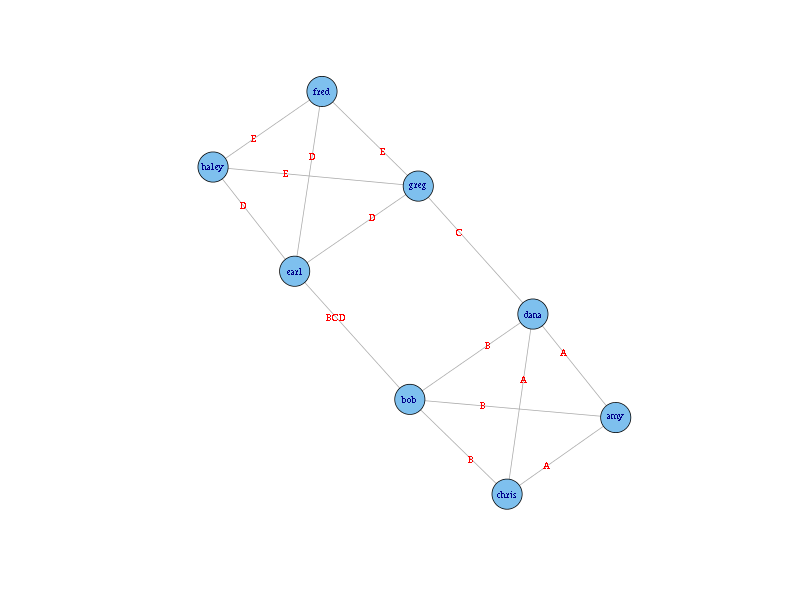
\includegraphics[width=0.65\linewidth]{toy2/orig.png}
  \caption{Original graph for Toy Dataset \#1.}
\end{figure}

Structural similarity only:

\begin{figure}[htp!]
  \centering
  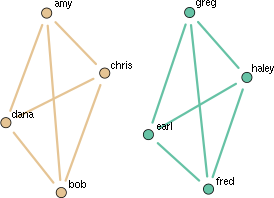
\includegraphics[width=0.65\linewidth]{toy2/no_ea/edge_comm.png}
  \caption{Communities using structural similarity only.}
\end{figure}

\begin{figure}[htp!]
  \centering
  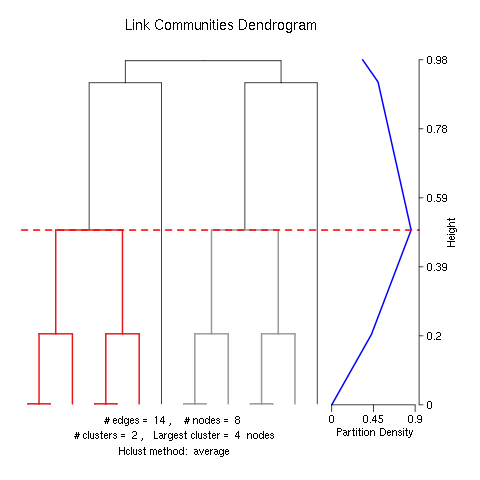
\includegraphics[width=0.65\linewidth]{toy2/no_ea/lc.png}
  \caption{Link communities dendogram using structural similarity only.}
\end{figure}

Structural similarity and edge attribute similarity:

\begin{figure}[htp!]
  \centering
  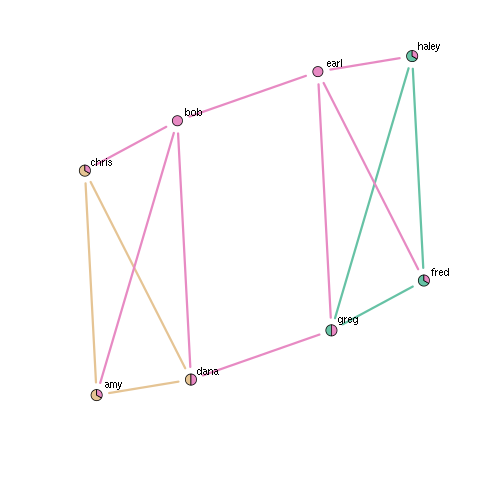
\includegraphics[width=0.65\linewidth]{toy2/ea/edge_comm_0.1.png}
  \caption{Communities using both, 10 percent structural.}
\end{figure}

\begin{figure}[htp!]
  \centering
  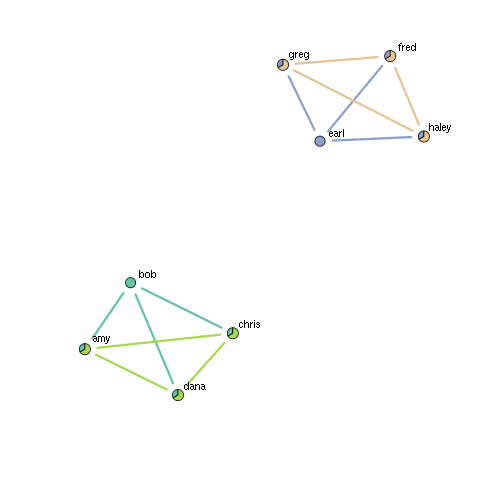
\includegraphics[width=0.65\linewidth]{toy2/ea/edge_comm_0.25.png}
  \caption{Communities using both, 25 percent structural.}
\end{figure}

\begin{figure}[htp!]
  \centering
  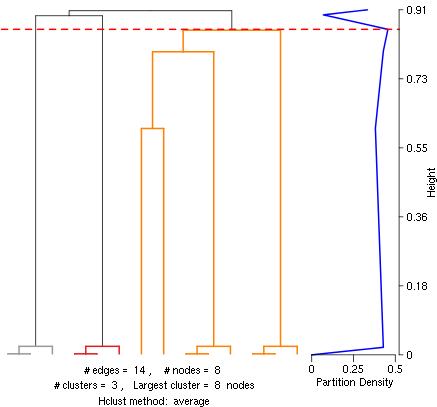
\includegraphics[width=0.65\linewidth]{toy2/ea/lc_0.1.png}
  \caption{Link communities dendogram using both, 10 percent structural.}
\end{figure}

\begin{figure}[htp!]
  \centering
  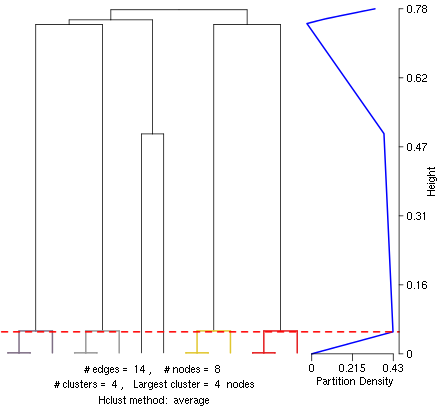
\includegraphics[width=0.65\linewidth]{toy2/ea/lc_0.25.png}
  \caption{Link communities dendogram using both, 25 percent structural.}
\end{figure}

\begin{figure}[htp!]
  \centering
  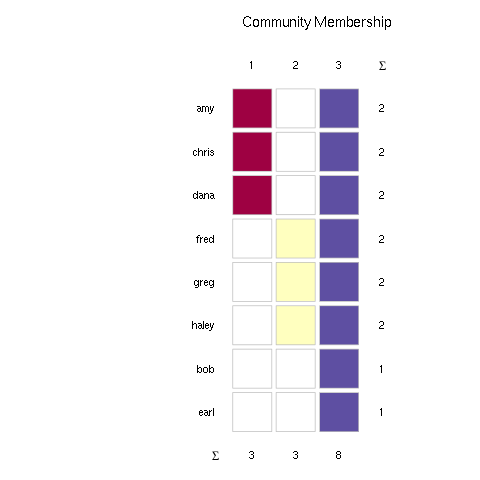
\includegraphics[width=0.65\linewidth]{toy2/ea/top20_0.1.png}
  \caption{Community membership using both, 10 percent structural.}
\end{figure}

\begin{figure}[htp!]
  \centering
  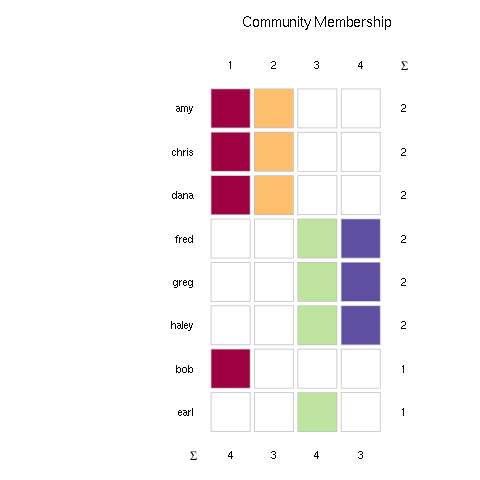
\includegraphics[width=0.65\linewidth]{toy2/ea/top20_0.25.png}
  \caption{Community membership using both, 25 percent structural.}
\end{figure}




\subsection*{Toy Dataset \#2}

\begin{figure}[htp!]
  \centering
  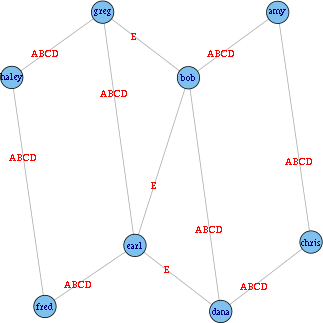
\includegraphics[width=0.65\linewidth]{toy3/orig.png}
  \caption{Original graph for toy Dataset \#2.}
\end{figure}


Structural similarity only:

\begin{figure}[htp!]
  \centering
  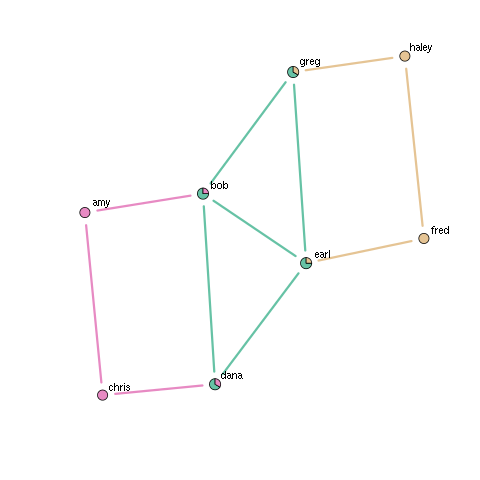
\includegraphics[width=0.65\linewidth]{toy3/no_ea/edge_comm.png}
  \caption{Communities using structural similarity only.}
\end{figure}

\begin{figure}[htp!]
  \centering
  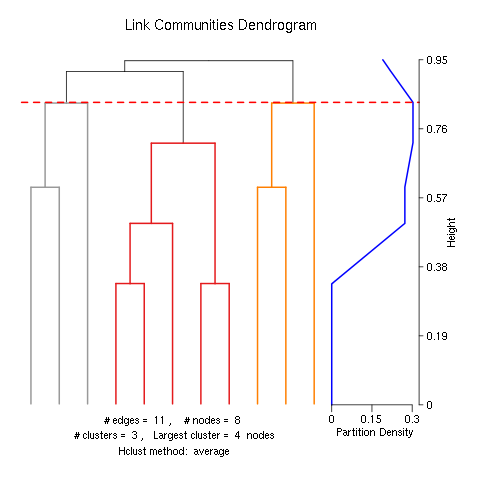
\includegraphics[width=0.65\linewidth]{toy3/no_ea/lc.png}
  \caption{Link communities dendogram using structural similarity only.}
\end{figure}

\begin{figure}[htp!]
  \centering
  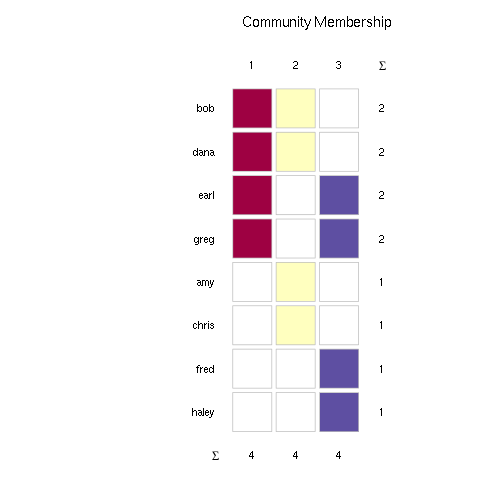
\includegraphics[width=0.65\linewidth]{toy3/no_ea/top20.png}
  \caption{Community membership using structural similarity only.}
\end{figure}

Structural similarity and edge attribute similarity:


\begin{figure}[htp!]
  \centering
  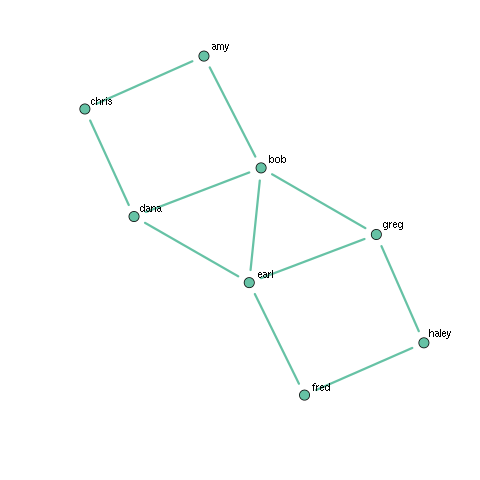
\includegraphics[width=0.65\linewidth]{toy3/ea/edge_comm_0.25.png}
  \caption{Communities using both. Unchanged from 10\% to 90\%.}
\end{figure}

\begin{figure}[htp!]
  \centering
  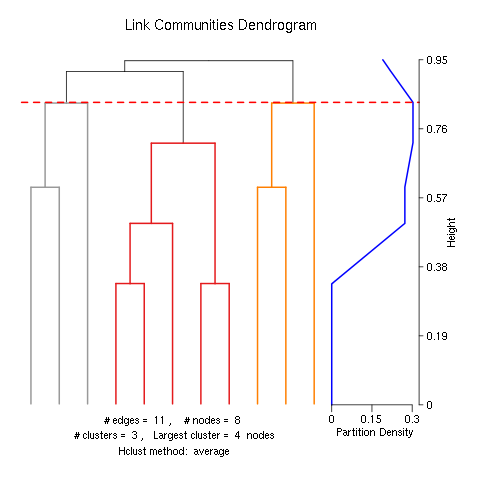
\includegraphics[width=0.65\linewidth]{toy3/no_ea/lc.png}
  \caption{Link communities dendogram both, 25\% structural.}
\end{figure}

\section*{Conclusions}

New approach may be appropriate if wish to cluster according to both link structure and edge attributes.\\

Limitations: In some cases, result is highly depend on chosen alpha value. In others, edge attributes are more influential in similarity measure, despite chosen alpha value. In both cases, it is necessary to choose the cutoff threshold for determining communities.

\nocite{DBLP:journals/corr/abs-1201-6568}
\nocite{ahn-lehmann-link-communities-nature-2010}
\nocite{Salem:2013:MMF:2500863.2500869}

\bibliography{references}
\bibliographystyle{unsrt}

\end{document}

%%% Local Variables: 
%%% mode: latex
%%% TeX-master: t
%%% End: 
